\chapter{Modelagem e Simulação} \label{cap3}

Neste capítulo será descrita a modelagem do sistema, o processo de estimação de velocidade do vento e a simulação do túnel de vento no Simulink Matlab.

\section{Descrição da Planta}
O sistema em questão, figura \ref{fig:tuneldevento}, se trata de um tubo PVC medindo de 40 mm de diâmetro e 120 cm de comprimento, afixado em uma plataforma plástica através de uma base e de elásticos para estabilização. Na extremidade inferior do tubo, encontra-se uma turbina de avião RC que empurra o ar para dentro do tubo elevando uma bola de tênis de mesa. Na extremidade superior, encontra-se um sensor infravermelho de distância. A turbina é controlada por um Arduino Mega 2560.

\begin{figure}
	\centering
	\includegraphics[width=0.3\linewidth]{pasta1_figuras/tuneldevento}
	\caption[Túnel de vento construído]{Túnel de vento construído}
	\label{fig:tuneldevento}
\end{figure}


\section{Modelo Matemático}


\begin{figure}[htb]
	\centering
	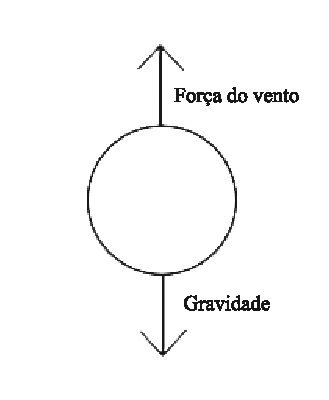
\includegraphics[width=0.3\linewidth]{pasta1_figuras/forcasatuantes}
	\caption[Forças atuantes na bola]{Forças atuantes na bola}
	\label{fig:forcasatuantes}
\end{figure}



Na figura \ref{fig:forcasatuantes} vemos que há duas forças atuantes na esfera: a gravidade que a puxa para baixo e a força de empuxo gerada pelo vento. Obtemos a seguinte equação do movimento,como visto em \cite{jernigan2009}:
\begin{equation}
m \ddot{h}=F=\dfrac{1}{2} \cdot C_a \cdot\rho \cdot A \cdot (v_{ar}- \dot{h})^2-m\cdot g
\end{equation}

onde $m$ é a massa da esfera, $h$ é a posição vertical da esfera no tubo, $\rho$ é a densidade do ar, $A$ é a área da esfera em contato com o fluxo de ar, $v_{ar}$ é a velocidade do ar dentro do tubo e $C_a$ é o coeficiente aerodinâmico da esfera. O coeficiente aerodinâmico depende da velocidade relativa entre a esfera e o vento, mas para as velocidades baixas de vento que estamos utilizando, esse valor pode ser considerado constante. Consideramos $\alpha= \dfrac{1}{2} \cdot C_a \cdot \rho \cdot A$:


\begin{equation} \label{eq:modelo}
\ddot{h}=\dfrac{\alpha}{m}\cdot (v_{ar}-\dot{h})^2-g
\end{equation}

\section{Estimação da Velocidade do Vento}

Para criarmos um simulador do sistema conforme descrito anteriormente, precisamos saber o valor de $v_{ar}$. Ele determina a velocidade do vento para diferentes valores de tensão e altura da bola. Não foi possível adquirir um sensor de velocidade do ar devido a problemas de localização geológica, portanto, foi necessário usar diferentes estratégias para adquirir a velocidade do ar em diversas alturas.


Foram adquiridas diversas bolas de tênis de mesa e se injetou uma mistura de cola e água nelas para aumentar o seu peso. Foram escolhidos 6 pesos diferentes e medidos em balança com precisão de duas casas decimais. Então para cada peso foi medida a tensão necessária para que se alcançasse as 6 alturas dentro da região de funcionamento do sensor, 10, 20, 30, 40, 50, 60 cm. Tendo medido a altura e a tensão necessária para alcançar as alturas, bastou utilizar a equação \eqref{eq:modelo} fazendo $\ddot{h}=\dot(h)=0$, obtendo-se a equação \ref{eq:varx} para calcular a velocidade do vento relacionada com uma altura e uma tensão.

\begin{equation}\label{eq:varx}
v_{ar}=\sqrt{\dfrac{gm}{\alpha}}
\end{equation}

Na figura \ref{fig:curvavar}, vemos a superfície gerada com os dados medidos. E a partir da função dessa superfície geramos a figura \ref{fig:graficovairaltura1} e a tabela \ref{tb:varxalturapwm}.

\begin{figure}[htb]
	\centering
	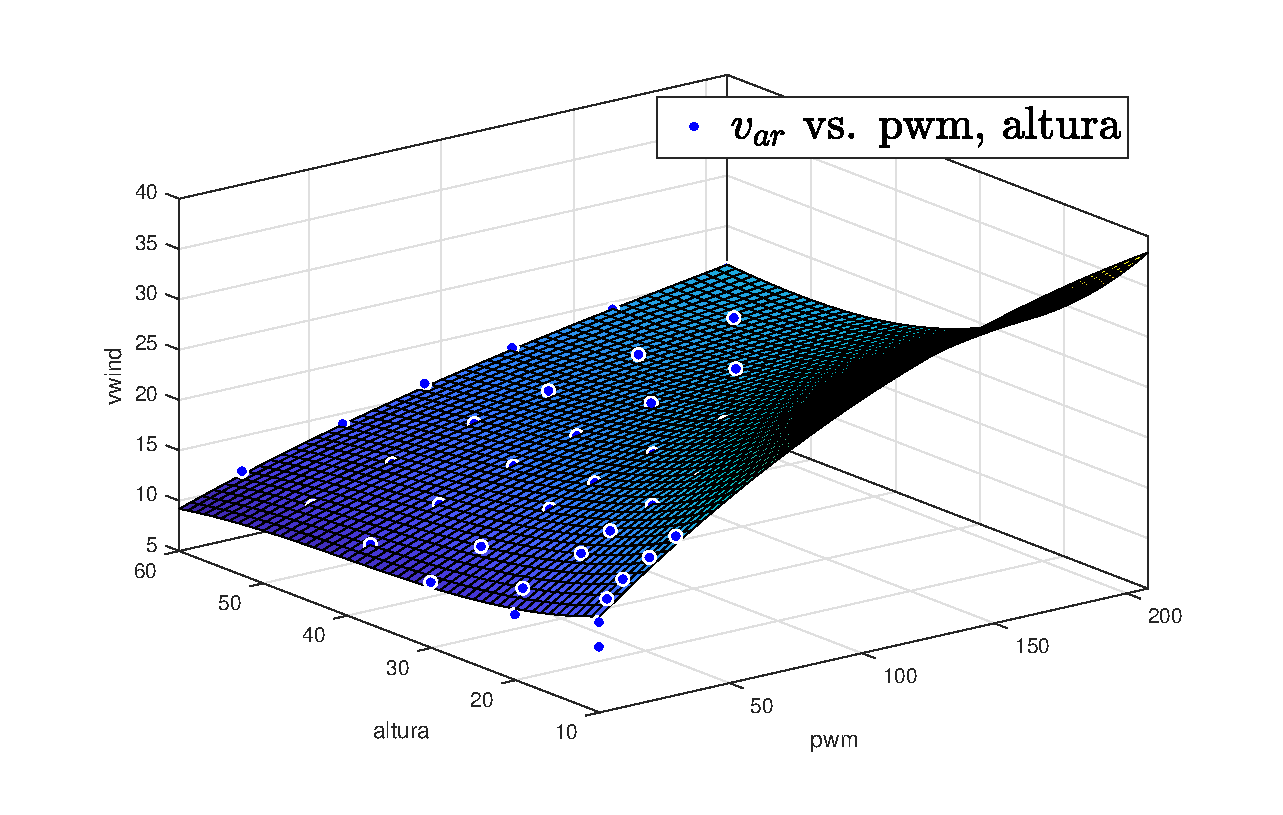
\includegraphics[width=1\linewidth]{pasta1_figuras/curvavar}
	\caption[Superfície de $v_{ar}$ em função de altura e pwm]{Superfície de $v_{ar}$ em função de altura e pwm}
	\label{fig:curvavar}
\end{figure}


\begin{figure}[htb]
	\centering
	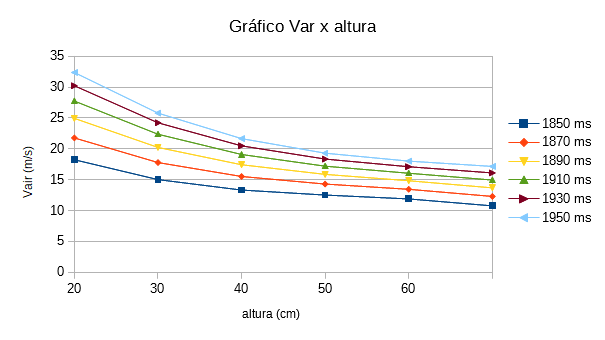
\includegraphics[width=1\linewidth]{grafico_vair_altura}
	\caption[Gráfico $v_{ar}$ x altura]{Gráfico de $v_{ar}$ x altura}
	\label{fig:graficovairaltura1}
\end{figure}

Podemos ver que a figura \ref{fig:graficovairaltura1} lembra um gráfico similar ao encontrado em \cite{jernigan2009} onde o autor utiliza um sensor de velocidade de vento e mostra uma curva similar, para uma mesma tensão aplicada na turbina. Quanto mais elevada se encontra a bola, menor vai ser a velocidade do ar que se choca com ela.

\begin{table}[htb]
	\centering
\begin{tabular}{|c|c|c|c|c|c|c|}
	\hline 
	Altura$\setminus$PWM & 1850 ms & 1870 ms & 1890 ms & 1910 ms & 1930 ms & 1950 ms \\ 
	\hline 
	10 cm & 18.24 & 21.78 & 24.94 & 27.75 & 30.22 & 32.37 \\ 
	\hline 
	20 cm & 15.02 & 17.79 & 20.24 & 22.38 & 24.23 & 25.80 \\ 
	\hline 
	30 cm & 13.33 & 15.52 & 17.44 & 19.09 & 20.49 & 21.67 \\ 
	\hline 
	40 cm & 12.51 & 14.30 & 15.86 & 17.21 & 18.35 & 19.30 \\ 
	\hline 
	50 cm & 11.88 & 13.45 & 14.84 & 16.05 & 17.11 & 18.03 \\ 
	\hline 
	60 cm & 10.76 & 12.29 & 13.68 & 14.95 & 16.10 & 17.16 \\ 
	\hline 
\end{tabular} 
\caption{Tabela da velocidade do ar em função de altura e do PWM aplicado ao motor}
\label{tb:varxalturapwm}
\end{table}

\section{Simulação do Túnel de Vento no Simulink}

Criamos um modelo de simulação( figura \ref{fig:simulador}) a partir da equação \ref{eq:modelo} e utilizamos os dados adquiridos em \ref{fig:graficovairaltura1} para fazer um ajuste de curva que alimenta o modelo com os valores da velocidade do vento para determinada altura e tensão no motor.

\begin{figure}[htb]
	\centering
	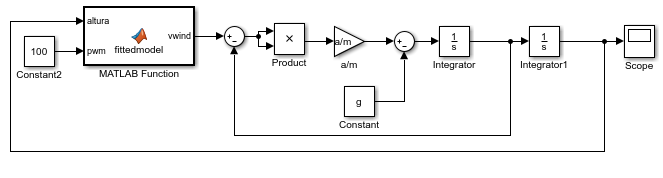
\includegraphics[width=1\linewidth]{simulador}
	\caption[Simulador do túnel de vento]{Simulador do túnel de vento}
	\label{fig:simulador}
\end{figure}

\begin{figure}[htb]
	\centering
	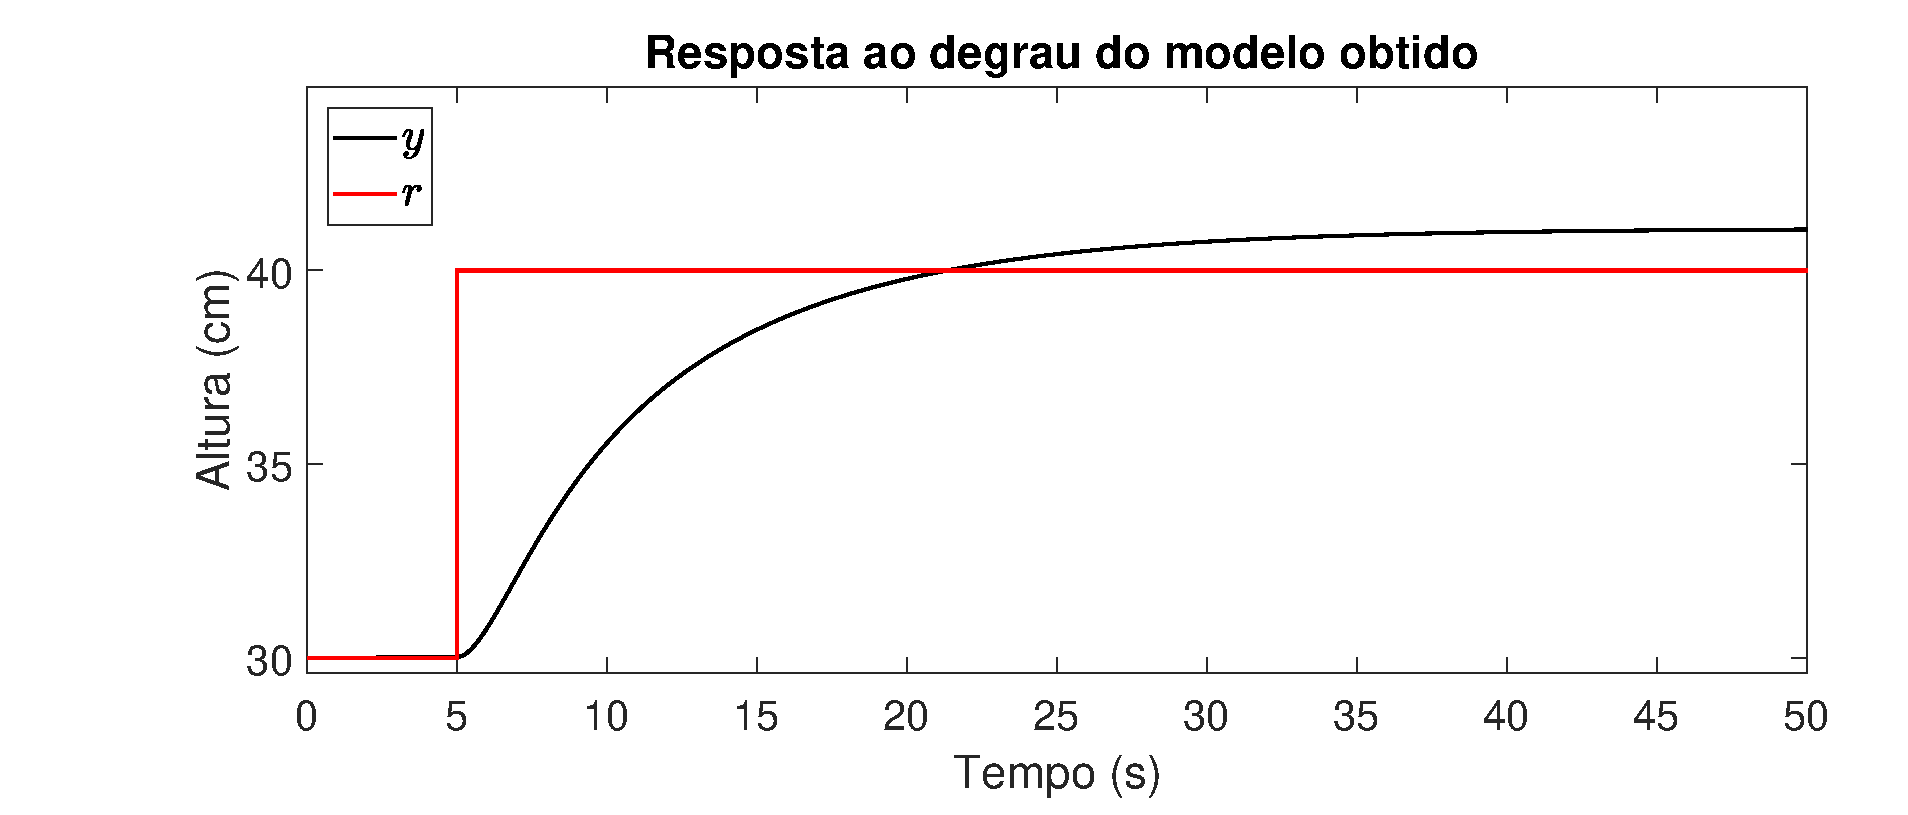
\includegraphics[width=1\linewidth]{pasta1_figuras/step_simul}
	\caption[Resposta ao degrau do simulador]{Resposta ao degrau do simulador}
	\label{fig:stepsimul}
\end{figure}

Na figura \ref{fig:stepsimul}, vemos como a resposta do simulador não representa o sistema real. O tempo de estabilização é 10 vezes maior que o tempo do sistema, mas o sobrevalor está condizente com o medido.



% Fim Capítulo
